\chapter{Mudança global e biosfera}\label{ch:b2:global-change}

Entre 1851 e 1858, Henry Thoreau percorreu os bosques e os prados em
torno de Concord, em Massachusetts, e anotou o dia em que cada uma de
cerca de quinhentas plantas floresceu pela primeira vez. Um século e meio
depois, botânicos voltaram aos mesmos lugares com seus cadernos. O
mirtilo-gigante que Thoreau via abrir em 11 de maio agora abre em
12 de abril; a flora inteira floresce, em média, dez dias mais cedo que
em sua época, acompanhando uma primavera \qty{2.4}{\celsius}
mais quente; e um quarto de suas espécies desapareceu de Concord --- não
ao acaso, mas justamente aquelas cuja floração não conseguiu acompanhar
a temperatura. Os capítulos anteriores forneceram a maquinaria: os ciclos
do \cref{ch:b2:biogeochemical-cycles}, a seleção e a deriva do
\cref{ch:b2:population-genetics}, a competição e a especiação
do \cref{ch:b2:speciation}, os \omterm{def:b2:living-soil:soil}{solos} do \cref{ch:b2:living-soil}.
Este capítulo põe números no que está acontecendo com os seres vivos
enquanto uma única espécie muda a química do ar e do mar: quanto
aquecimento por tonelada de carbono, quantos dias de primavera por grau,
quantos metros encosta acima, quanto ácido no mar, quantas espécies
perdidas por hectare --- e o que os números dizem sobre o século que
vem.

\section{A mudança física}

\begin{proposition}[O aquecimento é proporcional às emissões acumuladas]\label{prop:b2:global-change:tcre}
\index{aquecimento global}\index{emissões acumuladas}\index{orçamento de carbono}\index{efeito estufa}
O dióxido de carbono absorve o infravermelho emitido pelo \omterm{def:b2:living-soil:soil}{solo} e devolve
uma parte dele; mais \ensuremath{\mathrm{CO_2}} significa uma superfície mais quente, em cerca de
\qty{3}{\celsius} para cada duplicação, depois que os oceanos se ajustam
(a \emph{sensibilidade climática}). Como a resposta da temperatura
ao \ensuremath{\mathrm{CO_2}} é logarítmica na concentração, enquanto a \omterm{prop:b2:biogeochemical-cycles:carbon}{fração
atmosférica} das emissões cai à medida que a concentração sobe, as duas
curvaturas quase se anulam, e o aquecimento médio global é, numa boa
aproximação, \emph{linear na quantidade acumulada de
carbono emitido}, qualquer que seja o calendário:
\[
\Delta T \approx \lambda\,C_{\text{acum}}, \qquad \lambda \approx
\qty{1.65}{\celsius} \text{ por } \qty{1000}{GtC}
\]
(\qty{0.45}{\celsius} por \qty{1000}{Gt} de \ensuremath{\mathrm{CO_2}}). Cerca de
\qty{700}{GtC} emitidos desde 1850 aqueceram o planeta em
\qty{1.2}{\celsius} --- e a relação dá a cada meta um orçamento:
\qty{1.5}{\celsius} permite cerca de \qty{900}{GtC} no total,
\qty{200}{GtC} a mais do que já foi emitido, vinte anos no ritmo atual.
O aquecimento é desigual: o dobro da média sobre os continentes e o
triplo no Ártico; mais nas noites que nos dias; e ele vem acompanhado do
resto --- chuvas mais intensas e secas mais longas, um nível do mar que
sobe \qty{4}{mm} por ano, um gelo marinho um quinto menor no verão, e um
oceano que absorveu \qty{90}{\%} do calor e um quarto do carbono.
\end{proposition}
\begin{proof}[Evidências]
A proporcionalidade foi encontrada em modelos climáticos de todos os
graus de complexidade e confirmada pelo registro observado: o gráfico do
aquecimento desde 1850 em função das \omterm{prop:b2:global-change:tcre}{emissões acumuladas} dá uma reta ao
longo das décadas. O próprio \omterm{prop:b2:global-change:tcre}{efeito estufa} é medido a partir da órbita:
os satélites veem o infravermelho que a Terra emite com as bandas de
absorção do \ensuremath{\mathrm{CO_2}}, do metano e do vapor de água recortadas,
e o recorte se aprofundou entre 1970 e 2020 exatamente na medida que o
aumento desses gases prevê. Os isótopos e a queda do oxigênio do
\cref{ch:b2:biogeochemical-cycles} ligam o
\ensuremath{\mathrm{CO_2}} adicional aos combustíveis fósseis.
\end{proof}

\begin{omfigure}
\begin{tikzpicture}
\begin{axis}[
  width=0.88\linewidth, height=5.6cm,
  axis x line=bottom, axis y line=left,
  xmin=1845, xmax=2030, ymin=-0.3, ymax=1.5,
  xlabel={década}, ylabel={aquecimento (\unit{\celsius}) desde 1850--1900},
  xlabel style={font=\small, at={(axis description cs:0.5,-0.13)}, anchor=north},
  ylabel style={font=\small},
  tick label style={font=\small}, xtick={1850,1900,1950,2000}, ytick={0,0.5,1,1.5},
  scaled x ticks=false, x tick label style={/pgf/number format/1000 sep=},
  clip=false,
]
\addplot[ybar, bar width=7pt, fill=omThm!50, draw=omThm] coordinates {
(1855,0.00) (1865,-0.04) (1875,0.02) (1885,-0.06) (1895,-0.02) (1905,-0.10) (1915,-0.06) (1925,0.05) (1935,0.15) (1945,0.25) (1955,0.15) (1965,0.15) (1975,0.18) (1985,0.40) (1995,0.55) (2005,0.78) (2015,1.02) (2023,1.28)};
\node[font=\scriptsize, anchor=west, align=left] at (axis cs:1850,1.2) {cada barra: a média de uma década; a última, 2020--2024\\ \qty{700}{GtC} emitidos, $\qty{1.65}{\celsius}/\qty{1000}{GtC}$: \qty{1.2}{\celsius}};
\end{axis}
\end{tikzpicture}

{\small Temperatura média global da superfície por década, em relação à
segunda metade do século XIX. Cada uma das quatro últimas décadas bateu
um recorde, e a elevação desde 1970 é de \qty{0.2}{\celsius} por
década.}
\end{omfigure}

\section{O calendário: a fenologia}

\begin{theorem}[Graus-dia e a antecipação da primavera]\label{thm:b2:global-change:phenology}
\index{fenologia}\index{graus-dia}\index{tempo térmico}\index{descompasso fenológico}
Muitos eventos da vida das plantas e dos ectotérmicos --- a abertura dos
botões, a floração, a eclosão dos ovos, a emergência --- ocorrem quando
o \emph{\omterm{thm:b2:global-change:phenology}{tempo térmico}} acumulado desde uma data inicial, a soma das
temperaturas diárias acima de uma base $T_b$ (os \emph{graus-dia}),
atinge um total fixo $K$. Se a temperatura da primavera sobe linearmente, $T(t) = T_b
+ b\,(t - t_0)$, a $b$ graus por dia a partir do dia $t_0$ em que ela
cruza a base, o evento ocorre em
\[
t^{*} = t_0 + \sqrt{2K/b},
\]
e um aquecimento uniforme de $\Delta T$ antecipa o dia do cruzamento
em $\Delta T/b$, e o evento junto com ele: com $b \approx
\qty{0.1}{\celsius}$ por dia, \emph{cerca de dez dias mais cedo por
grau}. As espécies diferem em $T_b$, em $K$ e em usarem ou não também o
comprimento do dia, que o aquecimento não muda --- de modo que os membros
de uma cadeia alimentar se antecipam em ritmos diferentes e seus
calendários se desencontram: um \emph{\omterm{thm:b2:global-change:phenology}{descompasso fenológico}} entre a
lagarta e a ave que precisa alimentar seus filhotes com ela.
\end{theorem}
\begin{proof}
Graus-dia a partir de $t_0$: $\int_{t_0}^{t}(T - T_b)\,\mathrm{d}t' =
b\,(t - t_0)^{2}/2$, igual a $K$ quando $t - t_0 = \sqrt{2K/b}$.
Aquecer em $\Delta T$ substitui $T$ por $T + \Delta T$: a base é
cruzada $\Delta T/b$ dias mais cedo e a acumulação, idêntica a partir
desse dia, se completa $\Delta T/b$ dias mais cedo. (Se o aquecimento
também tornar $b$ mais íngreme, o intervalo $\sqrt{2K/b}$ também
encurta.) Uma espécie guiada pelo comprimento do dia mantém sua data;
uma guiada pelos graus-dia se desloca; a defasagem entre elas cresce em $\Delta T/b$.
\end{proof}
\begin{proof}[Evidências]
A flora de Concord de Thoreau e o registro da família Marsham de
vinte e sete sinais da primavera em Norfolk, mantido de 1736 a 1947,
mostram ambos a floração e a folheação se antecipando
\qtyrange{3}{6}{d} por grau de aquecimento da primavera. A floração das
cerejeiras de Kyoto, datada em diários da corte desde o século IX,
manteve-se em meados de abril durante mil anos e passou para o início de
abril desde 1900, com as datas mais precoces já registradas caindo nos
anos 2020. Nos Países Baixos, as lagartas dos carvalhos atingem hoje seu
pico duas semanas mais cedo que em 1985; o chapim-real, guiado pelo
mesmo calor, acompanhou o ritmo, mas o papa-moscas-preto, que regula sua
migração a partir da África pelo comprimento do dia, chega como antes e
encontra o pico já passado --- suas populações caíram \qty{90}{\%} onde o
descompasso é maior (Both e colaboradores, 2006).
\end{proof}

\begin{omfigure}
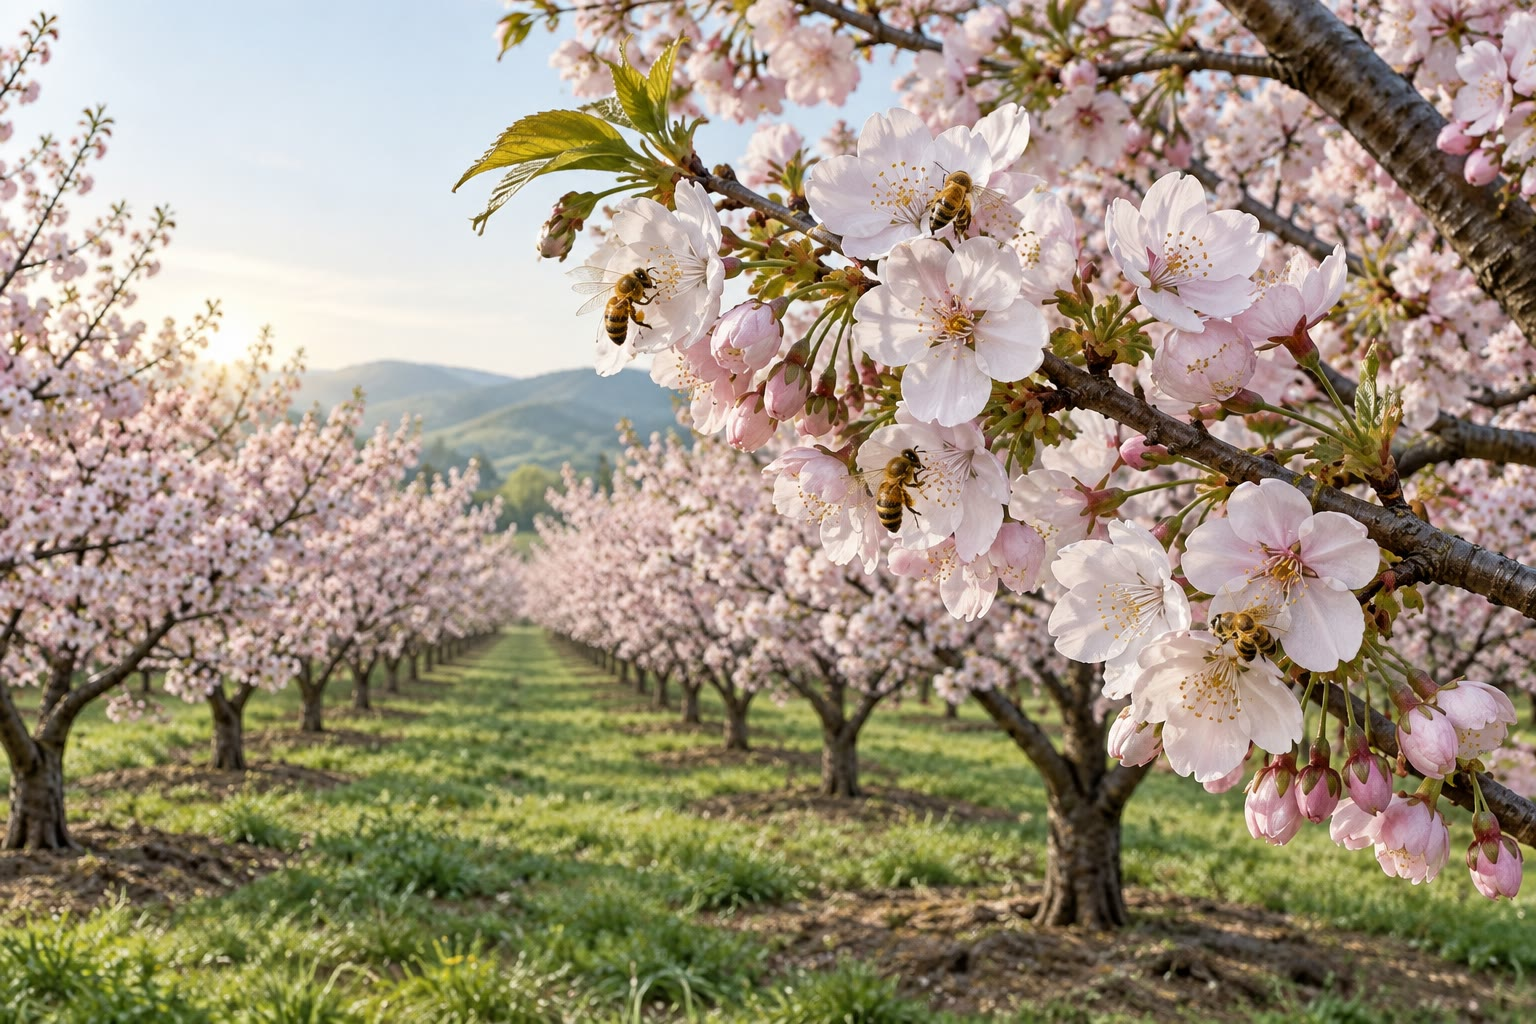
\includegraphics[width=0.62\linewidth]{images/book4/ai/b4-27-phenology-cherry.jpg}

{\small Um pomar de cerejeiras em flor. As cerejeiras de Kyoto, datadas
em diários durante doze séculos, abrem agora mais cedo que em qualquer
ano anterior a 1900 --- e as abelhas que as polinizam precisam estar
voando no mesmo dia.}
\end{omfigure}

\begin{omfigure}
\begin{tikzpicture}
\begin{axis}[
  width=0.74\linewidth, height=5.4cm,
  axis x line=bottom, axis y line=left,
  xmin=0, xmax=100, ymin=0, ymax=14,
  xlabel={dias a partir de 1\textsuperscript{o} de março}, ylabel={temperatura média diária (\unit{\celsius})},
  xlabel style={font=\small, at={(axis description cs:0.5,-0.13)}, anchor=north},
  ylabel style={font=\small},
  tick label style={font=\small}, xtick={0,20,40,60,80,100},
  legend style={font=\scriptsize, at={(0.03,0.97)}, anchor=north west, draw=none},
  clip=false,
]
\addplot[very thick, omDef, domain=0:100, samples=2] {2 + 0.1*x};
\addlegendentry{primavera antes do aquecimento}
\addplot[very thick, omThm, domain=0:100, samples=2] {3 + 0.1*x};
\addlegendentry{primavera \qty{1}{\celsius} mais quente}
\draw[dashed, gray] (axis cs:0,5) -- (axis cs:100,5); \node[font=\scriptsize, anchor=south east] at (axis cs:100,5) {temperatura de base $T_b = \qty{5}{\celsius}$};
\fill[omDef, opacity=0.15] (axis cs:30,5) -- (axis cs:93,5) -- (axis cs:93,11.3) -- cycle;
\fill[omThm, opacity=0.15] (axis cs:20,5) -- (axis cs:83,5) -- (axis cs:83,11.3) -- cycle;
\draw[<->, thick] (axis cs:83,1.6) -- (axis cs:93,1.6); \node[font=\scriptsize, anchor=south] at (axis cs:88,1.8) {10 dias};
\draw[dotted] (axis cs:93,0) -- (axis cs:93,5); \draw[dotted] (axis cs:83,0) -- (axis cs:83,5);
\node[font=\scriptsize, anchor=south, align=center] at (axis cs:62,11.4) {$K = 200$ graus-dia\\ (áreas sombreadas)};
\end{axis}
\end{tikzpicture}

{\small Graus-dia. O evento ocorre quando a área sombreada entre a reta
da temperatura e a base atinge $K$; uma primavera um grau mais quente
cruza a base dez dias antes e completa a soma dez dias antes.}
\end{omfigure}

\section{O mapa: deslocamentos de áreas de distribuição}

\begin{proposition}[As isotermas se deslocam, e as espécies as seguem]\label{prop:b2:global-change:range}
\index{deslocamento da área de distribuição}\index{velocidade climática}\index{gradiente térmico vertical}
A temperatura cai cerca de \qty{6.5}{\celsius} por quilômetro de
altitude e cerca de \qty{0.65}{\celsius} por cem quilômetros de latitude
na zona temperada; um aquecimento de \qty{1}{\celsius} desloca, portanto,
cada isoterma cerca de \qty{150}{m} encosta acima e
\qty{150}{km} em direção ao polo. As espécies cujos limites são fixados
pela temperatura se deslocam com sua isoterma, se puderem: a média de
centenas de espécies estudadas se deslocou \qty{11}{m} encosta acima e
\qty{17}{km} em direção ao polo por década desde 1970, na velocidade das
isotermas, e as mais rápidas --- móveis, generalistas, de vida curta ---
as ultrapassam, enquanto as árvores, cujas \omterm{def:b2:angiosperm-reproduction:seed}{sementes} viajam alguns metros
por ano, e as espécies que já estão no cume ou no polo não conseguem
acompanhar: o topo de uma montanha não tem para onde ir, e cada grau de
aquecimento elimina os \qty{150}{m} mais altos de cada área de
distribuição. As espécies marinhas, sem barreiras e com limites térmicos
mais estreitos, se deslocam mais depressa, dezenas de quilômetros por
década; o bacalhau, a cavala e as pescarias junto com eles se deslocaram
para o norte através de mares inteiros. A borda superior de uma área de
distribuição avança, a borda inferior recua à medida que esquenta e que
novos competidores chegam de baixo, e a comunidade em cada ponto é
remontada a partir de espécies que nunca se encontraram.
\end{proposition}
\begin{proof}[Evidências]
Parmesan (1996) refez o levantamento da borboleta \textit{Euphydryas
editha} em sua área de distribuição no oeste da América do Norte: as
populações da borda sul e das baixas altitudes estavam extintas, as da
borda norte e das grandes altitudes prosperavam, e a área inteira tinha
se deslocado \qty{92}{km} para o norte e \qty{124}{m} para cima --- a
primeira espécie da qual se mostrou que acompanhou as isotermas. Lenoir e
colaboradores (2008) compararam levantamentos de plantas florestais de
1905--1985 com os de 1986--2005 nas montanhas francesas: a altitude ótima
de 171 espécies tinha subido \qty{29}{m} por década. Chen e colaboradores
(2011), com duas mil espécies, encontraram deslocamentos duas a três
vezes mais rápidos que as estimativas anteriores, e proporcionais ao
aquecimento local.
\end{proof}

\begin{omfigure}
\begin{tikzpicture}[every node/.style={font=\scriptsize}, >=stealth]
  \fill[gray!25] (0,0) -- (3.5,4.2) -- (7,0) -- cycle;
  \draw[thick] (0,0) -- (3.5,4.2) -- (7,0);
  \foreach \y/\lab in {1.0/{\qty{12}{\celsius}}, 2.2/{\qty{8}{\celsius}}, 3.4/{\qty{4}{\celsius}}} { \draw[omDef, thick] ({\y/1.2},\y) -- ({7-\y/1.2},\y) node[right] {\lab}; }
  \foreach \y in {1.15,2.35,3.55} { \draw[omThm, thick, dashed] ({\y/1.2},\y) -- ({7-\y/1.2},\y); }
  \node[omThm, anchor=west, align=left] at (7.6,3.7) {tracejadas: as mesmas isotermas\\ após \qty{1}{\celsius} de aquecimento,\\ \qty{150}{m} mais acima};
  \fill[omProp!50] (0.83,1.0) -- (6.17,1.0) -- (5.17,2.2) -- (1.83,2.2) -- cycle;
  \node[align=center] at (3.5,1.6) {faixa de uma espécie,\\ \qtyrange{1000}{1200}{m}};
  \draw[->, thick, omExo!80!black] (1.1,2.2) -- (1.1,2.9); \node[omExo!80!black, anchor=east, align=right] at (0.95,2.55) {a faixa sobe\\ e encolhe};
  \node[anchor=north] at (3.5,-0.1) {uma montanha: a área diminui com a altitude, e o cume não tem para onde subir};
\end{tikzpicture}

{\small Um deslocamento de área de distribuição numa montanha. Cada grau
eleva as isotermas \qty{150}{m}; uma espécie acompanha sua faixa para
cima, numa área menor, e uma faixa que já está no cume se perde.}
\end{omfigure}

\section{O mar: acidificação e calor}

\begin{theorem}[Acidificação]\label{thm:b2:global-change:acid}
\index{acidificação dos oceanos}\index{sistema carbonato}\index{estado de saturação}\index{branqueamento dos corais}
O dióxido de carbono que se dissolve na água do mar forma ácido
carbônico, que se dissocia: $\ensuremath{\mathrm{CO_2}} + \ensuremath{\mathrm{H_2O}} \rightleftharpoons \ensuremath{\mathrm{H^{+}}} +
\ensuremath{\mathrm{HCO_3^{-}}}$, com $[\ensuremath{\mathrm{H^{+}}}][\ensuremath{\mathrm{HCO_3^{-}}}]/[\ensuremath{\mathrm{CO_2}}] = K_1$.
O bicarbonato é o maior estoque de carbono do oceano e é mantido quase
constante pela alcalinidade, de modo que
\[
[\ensuremath{\mathrm{H^{+}}}] \propto p_{\ensuremath{\mathrm{CO_2}}}, \qquad
\Delta\mathrm{pH} \approx -\log_{10}\frac{p_{\ensuremath{\mathrm{CO_2}}}}{p_0}
\]
--- mais precisamente $-0.9\log_{10}$ da razão, porque o bicarbonato
aumenta um pouco. De 280 para \qty{420}{ppm}, o pH superficial caiu
$0.15$, de $8.2$ para $8.05$: um aumento de \qty{40}{\%} dos íons
hidrogênio; a \qty{800}{ppm}, cairia $0.4$. Os íons hidrogênio adicionais
consomem carbonato, $\ensuremath{\mathrm{H^{+}}} + \ensuremath{\mathrm{CO_3^{2-}}} \to \ensuremath{\mathrm{HCO_3^{-}}}$, e
o \emph{\omterm{thm:b2:global-change:acid}{estado de saturação}} $\Omega$ do carbonato de cálcio ---
o produto das concentrações de cálcio e de carbonato dividido pelo
produto de solubilidade --- cai na mesma proporção: as conchas e os
esqueletos de aragonita (corais, pterópodes) se formam facilmente com $\Omega > 3$,
com dificuldade perto de 1, e se dissolvem abaixo disso; a superfície
tropical, com $\Omega \approx 4$ antes da indústria e 3 hoje, chega a 2
a \qty{560}{ppm}, e as águas superficiais polares, frias e ricas em
\ensuremath{\mathrm{CO_2}}, chegam a 1 primeiro.
\end{theorem}
\begin{proof}
A partir do equilíbrio, $[\ensuremath{\mathrm{H^{+}}}] = K_1[\ensuremath{\mathrm{CO_2}}]/[\ensuremath{\mathrm{HCO_3^{-}}}]$ e
$[\ensuremath{\mathrm{CO_2}}]$ é proporcional a $p_{\ensuremath{\mathrm{CO_2}}}$ pela lei de Henry;
com $[\ensuremath{\mathrm{HCO_3^{-}}}]$ constante, $[\ensuremath{\mathrm{H^{+}}}]$ é proporcional a
$p_{\ensuremath{\mathrm{CO_2}}}$ e $\mathrm{pH} = -\log_{10}[\ensuremath{\mathrm{H^{+}}}]$ varia de
$-\log_{10}$ da razão. O segundo equilíbrio, $[\ensuremath{\mathrm{H^{+}}}][\ensuremath{\mathrm{CO_3^{2-}}}]/[\ensuremath{\mathrm{HCO_3^{-}}}]
= K_2$, dá $[\ensuremath{\mathrm{CO_3^{2-}}}] \propto 1/[\ensuremath{\mathrm{H^{+}}}] \propto
1/p_{\ensuremath{\mathrm{CO_2}}}$, de modo que $\Omega$ cai quando $p_{\ensuremath{\mathrm{CO_2}}}$ sobe, e
o aumento de \qty{40}{\%} de $[\ensuremath{\mathrm{H^{+}}}]$ é uma queda de \qty{30}{\%} do
carbonato. (A química completa, com a variação do bicarbonato e as
atividades iônicas, dá o fator $0.9$ e os números observados; o volume
do Ano 3 a trata.)
\end{proof}
\begin{proof}[Evidências]
A estação oceânica ao norte do Havaí mede o pH superficial todos os meses
desde 1988: ele cai $0.0018$ por ano, acompanhando o
\ensuremath{\mathrm{CO_2}} de Mauna Loa, logo acima, como exige a química.
Os pterópodes --- os caracóis do mar, alimento de salmões e baleias ---
coletados ao largo da costa do Pacífico mostram suas conchas de aragonita
corroídas e se dissolvendo onde a ressurgência traz à superfície água
com $\Omega <
1$. O \omterm{thm:b2:global-change:acid}{branqueamento dos corais} é causado pelo calor, e não pelo ácido:
quando a água fica \qty{1}{\celsius} acima do máximo de verão durante
algumas semanas, o coral expulsa suas algas simbióticas e passa fome; a
Grande Barreira de Coral branqueou em 1998, 2002, 2016, 2017, 2020, 2022
e 2024, e metade de sua cobertura de corais desapareceu desde 1995.
\end{proof}

\begin{omfigure}
\begin{tikzpicture}
\begin{axis}[
  width=0.68\linewidth, height=5.4cm,
  axis x line=bottom, axis y line=left,
  xmin=250, xmax=1000, ymin=7.6, ymax=8.3,
  xlabel={\ensuremath{\mathrm{CO_2}} atmosférico (ppm)}, ylabel={pH superficial},
  xlabel style={font=\small, at={(axis description cs:0.5,-0.13)}, anchor=north},
  ylabel style={font=\small},
  tick label style={font=\small}, xtick={280,420,560,800,1000}, ytick={7.6,7.8,8.0,8.2},
  clip=false,
]
\addplot[very thick, omDef, domain=250:1000, samples=60] {8.2 - 0.9*log10(x/280)};
\fill[omDef] (axis cs:280,8.2) circle (2pt); \node[font=\scriptsize, anchor=south west] at (axis cs:285,8.2) {1750};
\fill[omThm] (axis cs:420,8.04) circle (2pt); \node[font=\scriptsize, anchor=south west] at (axis cs:425,8.04) {2020s: $-0.15$, $+\qty{40}{\%}$ \ensuremath{\mathrm{H^{+}}}};
\fill[omThm] (axis cs:800,7.79) circle (2pt); \node[font=\scriptsize, anchor=south west] at (axis cs:805,7.79) {2100 com emissões altas};
\node[font=\scriptsize, anchor=north east, align=right] at (axis cs:1000,8.28) {$\Omega_{\text{aragonita}}$, trópicos:\\ 4 em 1750, 3 hoje, 2 a \qty{560}{ppm}};
\end{axis}
\end{tikzpicture}

{\small pH da superfície do oceano em função do dióxido de carbono
atmosférico, $\mathrm{pH} = 8.2 - 0.9\log_{10}(p/280)$. A escala é
logarítmica: cada décimo de unidade representa um quarto a mais de íons
hidrogênio.}
\end{omfigure}

\begin{omfigure}
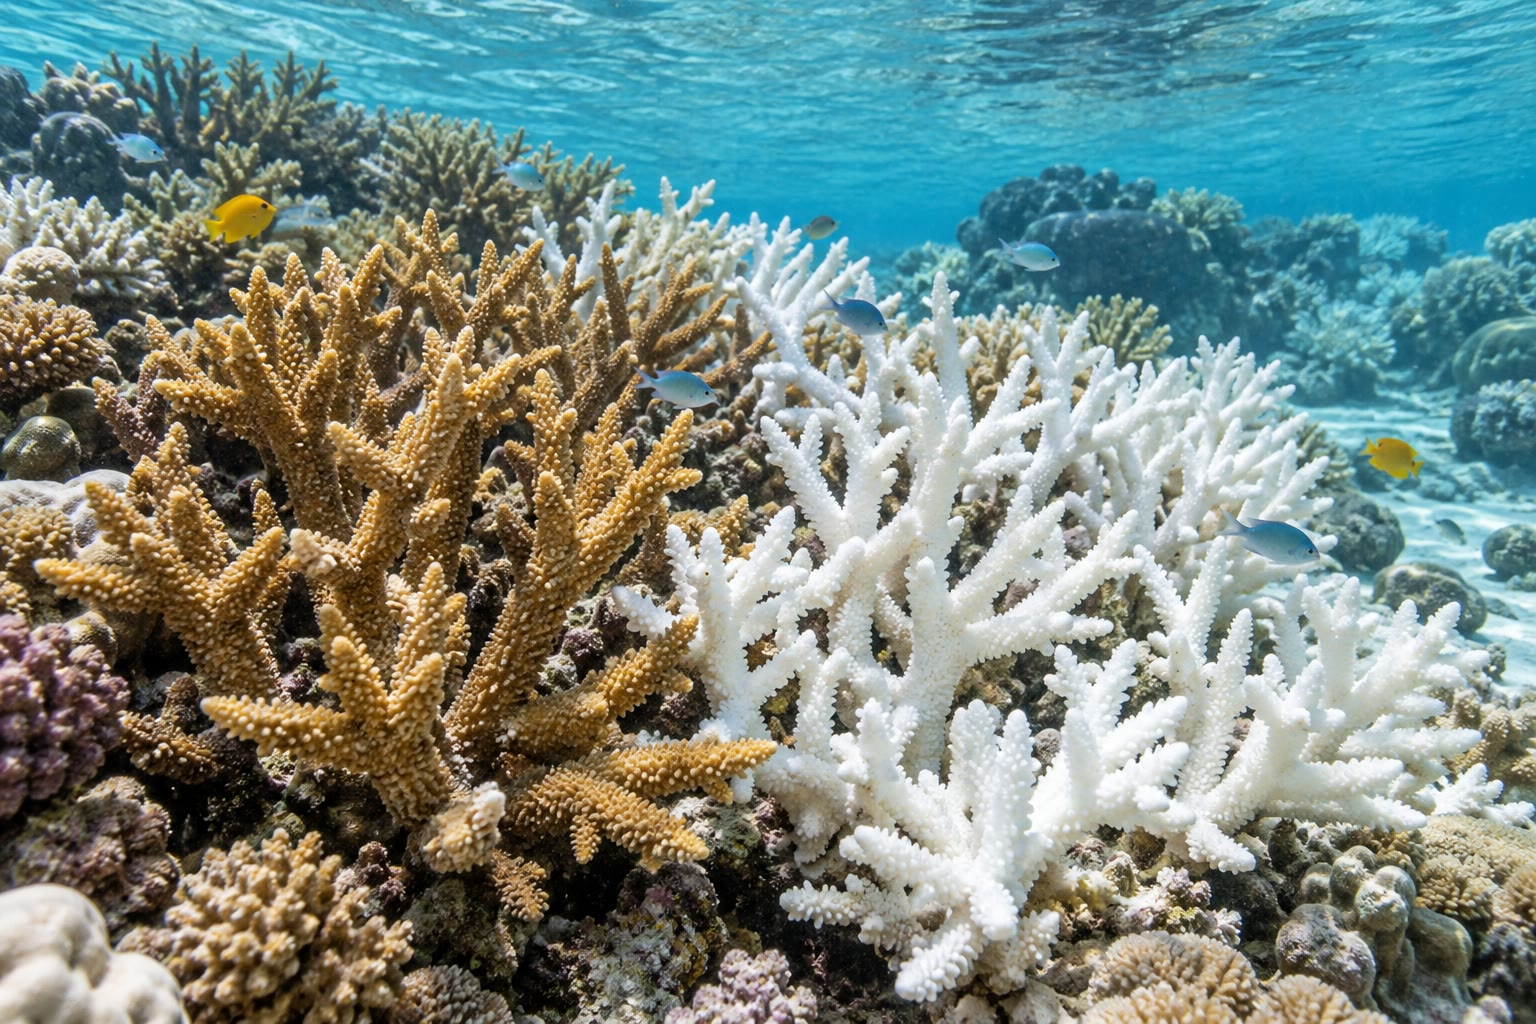
\includegraphics[width=0.44\linewidth]{images/book4/ai/b4-27-coral-bleaching.jpg}\hspace{0.04\linewidth}
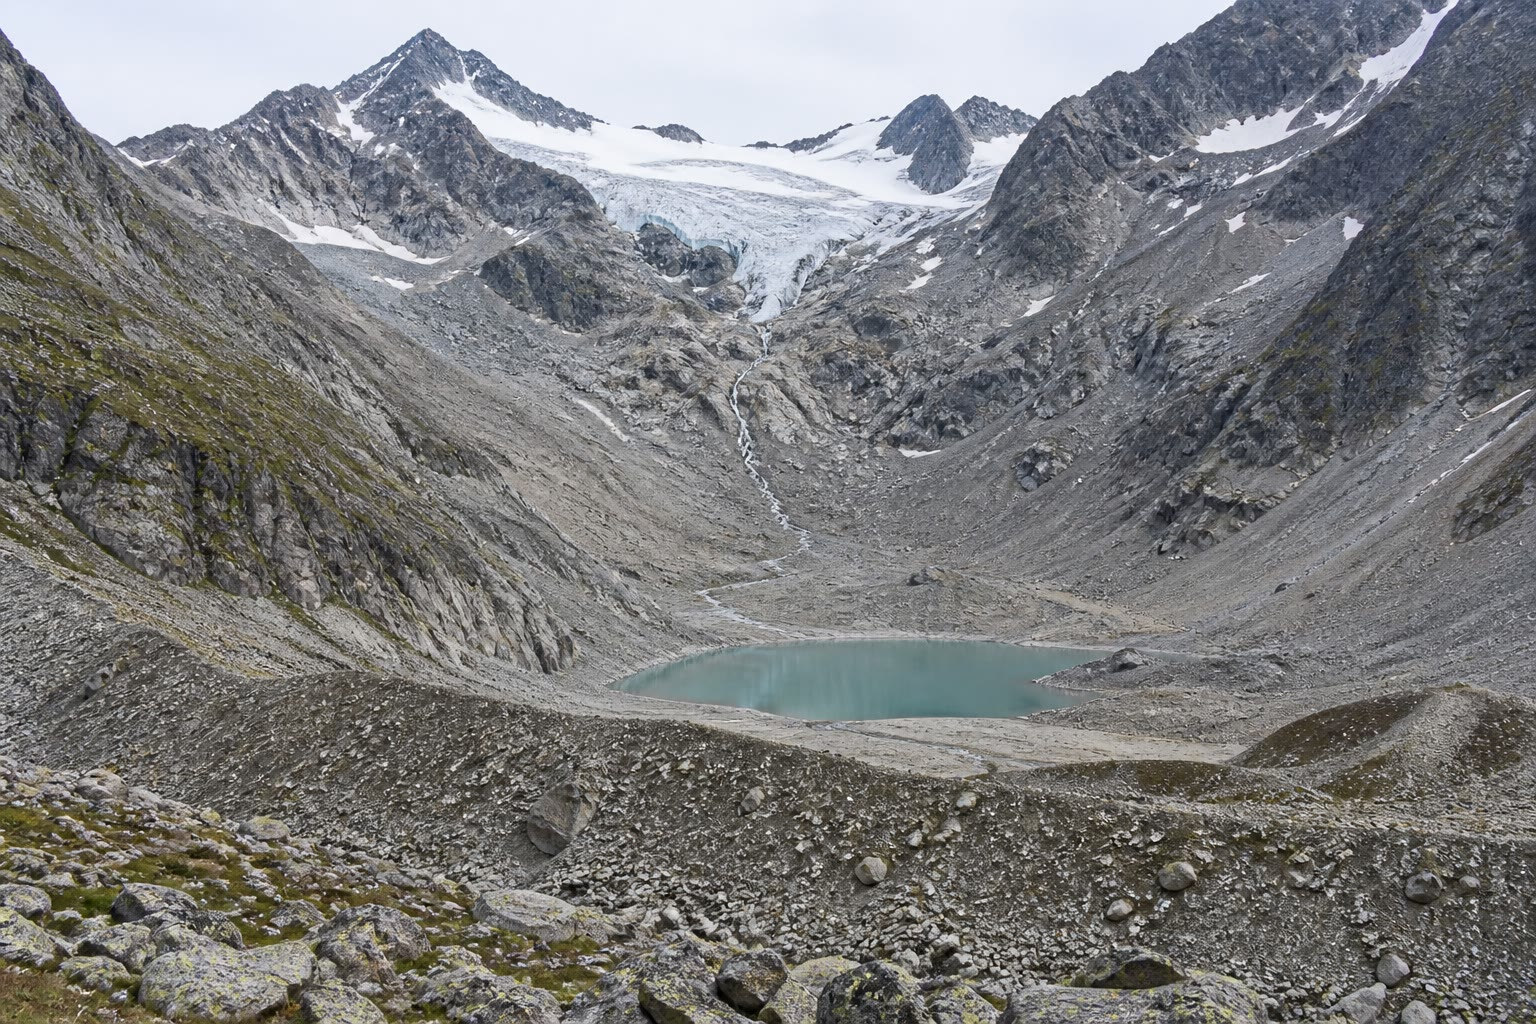
\includegraphics[width=0.44\linewidth]{images/book4/ai/b4-27-glacier-retreat.jpg}

{\small Dois termômetros. À esquerda: um recife branqueado, com o
esqueleto branco do coral aparecendo através do tecido que perdeu suas
algas. À direita: uma geleira de vale que recuou vale acima, deixando a
rocha nua onde havia gelo um século atrás.}
\end{omfigure}

\section{O livro-caixa: a extinção e sua estimativa}

\begin{theorem}[A relação espécie--área e o custo da perda de hábitat]\label{thm:b2:global-change:sar}
\index{relação espécie--área}\index{taxa de extinção}\index{perda de hábitat}\index{dívida de extinção}
O número de espécies encontradas numa área $A$ cresce como uma potência
da área, $S = cA^{z}$, com $z \approx 0.25$ para ilhas e fragmentos de
hábitat (dobrar a área acrescenta um quinto a mais de espécies; uma área
cem vezes maior, três vezes mais). Se um hábitat é reduzido a uma
fração $1 - h$ de sua extensão, o número de espécies que ele pode
finalmente abrigar cai para $(1 - h)^{z}$ do original: a perda de
metade do hábitat custa \qty{16}{\%} de suas espécies,
\qty{90}{\%} custam \qty{44}{\%}, e \qty{99}{\%} custam
\qty{68}{\%}. A perda não é imediata --- os sobreviventes do fragmento
persistem por um tempo, uma \emph{\omterm{thm:b2:global-change:sar}{dívida de extinção}} paga ao longo de
décadas à medida que as pequenas populações sucumbem à deriva e à
endogamia do \cref{ch:b2:population-genetics} --- e ela é a base da
estimativa de que a \omterm{thm:b2:global-change:sar}{taxa de extinção} atual é de cem a mil vezes a taxa
de fundo do registro fóssil: cerca de uma espécie em um milhão por ano,
contra os vários milhares por ano, de uns dez milhões, que se perdem
hoje.
\end{theorem}
\begin{proof}
$S'/S = (A'/A)^{z} = (1 - h)^{z}$; com $z = 0.25$, $0.5^{0.25} =
0.84$, $0.1^{0.25} = 0.56$, $0.01^{0.25} = 0.32$. A relação em si é
empírica; seu expoente reflete o equilíbrio, nas ilhas, entre a
imigração de novas espécies (que cai à medida que a ilha se enche) e a
extinção das residentes (que sobe à medida que suas populações encolhem
com a área), o equilíbrio da teoria de MacArthur e
Wilson.
\end{proof}
\begin{proof}[Evidências]
As ilhas do grupo do Krakatoa, esterilizadas pela erupção de 1883, foram
recolonizadas por plantas, aves e insetos numa sucessão que atingiu, em
cinquenta anos, os números de espécies previstos a partir de suas áreas;
as ilhotas de manguezal que Simberloff e Wilson fumigaram na Flórida em
1966 voltaram a seu número original de espécies, com espécies
diferentes, em um ano. A Mata Atlântica, reduzida a \qty{10}{\%} de sua
extensão, perdeu ou quase perdeu a fração de suas espécies de aves que a
relação prevê; e em todos os grupos avaliados pela União Internacional
para a Conservação da Natureza, de um quarto a um terço das espécies
estão ameaçadas --- aves \qty{13}{\%}, mamíferos \qty{27}{\%},
anfíbios \qty{41}{\%}, corais
\qty{44}{\%} ---, com a \omterm{thm:b2:global-change:sar}{perda de hábitat} como primeira causa, e a caça,
as \omterm{prop:b2:global-change:invasion}{espécies invasoras}, a poluição e, cada vez mais, o clima como as
outras.
\end{proof}

\begin{omfigure}
\begin{tikzpicture}
\begin{loglogaxis}[
  width=0.68\linewidth, height=5.4cm,
  axis x line=bottom, axis y line=left,
  xmin=1, xmax=100000, ymin=5, ymax=200,
  xlabel={área da ilha (\unit{km^2})}, ylabel={espécies de aves terrestres},
  xlabel style={font=\small, at={(axis description cs:0.5,-0.13)}, anchor=north},
  ylabel style={font=\small},
  tick label style={font=\small},
  clip=false,
]
\addplot[only marks, mark=*, mark size=2pt, omDef] coordinates {(1.5,9) (8,14) (35,22) (150,32) (400,37) (1200,52) (4000,70) (13000,92) (35000,125) (85000,160)};
\addplot[very thick, omThm, domain=1:100000, samples=2] {9*x^0.25};
\node[font=\scriptsize, omThm, anchor=north west, align=left] at (axis cs:2,120) {$S = 9A^{0.25}$: uma área cem\\ vezes maior, três vezes\\ mais espécies};
\end{loglogaxis}
\end{tikzpicture}

{\small A \omterm{thm:b2:global-change:sar}{relação espécie--área}, aqui para as aves terrestres das ilhas
de um arquipélago: uma reta de inclinação $z = 0.25$ em eixos
logarítmicos. Reduza um hábitat a um décimo e ele acabará conservando
pouco mais da metade de suas espécies.}
\end{omfigure}

\begin{proposition}[Invasões, serviços e o que pode ser feito]\label{prop:b2:global-change:invasion}
\index{espécie invasora}\index{serviços ecossistêmicos}\index{mitigação}\index{neutralidade líquida}
Navios, aviões e o comércio levaram milhares de espécies para além das
barreiras que as mantinham separadas; a maioria não consegue se
estabelecer, mas as poucas que conseguem --- o coelho na Austrália, o
mexilhão-zebra nos Grandes Lagos, a cobra-arbórea-marrom que esvaziou
Guam de suas aves, o fungo quitrídio que levou noventa espécies de
anfíbios à extinção --- se espalham como uma frente que avança a
velocidade constante, $c =
2\sqrt{rD}$ para uma população que cresce à taxa $r$ e se dispersa
com coeficiente de difusão $D$ (o rato-almiscarado de Skellam, solto
perto de Praga em 1905, expandiu-se pela Europa a \qty{11}{km} por ano,
com o raio de sua área de distribuição crescendo em linha reta com o
tempo). Diante de tudo isso está o que a biosfera faz por sua única
espécie problemática: a \omterm{def:b2:angiosperm-reproduction:pollination}{polinização} de três quartos das culturas, a
purificação da água, o controle das cheias, a fixação do nitrogênio e a
formação do \omterm{def:b2:living-soil:soil}{solo}, as pescarias, o carbono guardado nas florestas e nos
\omterm{def:b2:living-soil:soil}{solos} --- \emph{\omterm{prop:b2:global-change:invasion}{serviços ecossistêmicos}} avaliados, onde se pode
pôr-lhes um preço, em mais que o produto econômico mundial. O que pode
ser feito decorre dos números. O aquecimento para quando as emissões
líquidas param, e não antes: os \omterm{thm:b2:biogeochemical-cycles:box}{modelos de caixa} do
\cref{ch:b2:biogeochemical-cycles} não permitem outra leitura da
\emph{\omterm{prop:b2:global-change:invasion}{neutralidade líquida}}. As terras podem ajudar dentro de certos
limites --- uma gigatonelada de carbono por ano, vinda do
reflorestamento e dos \omterm{def:b2:living-soil:soil}{solos}, durante algumas décadas, contra dez vindas
dos combustíveis fósseis --- e as espécies podem ser ajudadas a se
deslocar, ou mantidas em reservas grandes e conectadas o bastante para
que a \omterm{thm:b2:global-change:sar}{relação espécie--área} e a deriva das pequenas populações não
acabem com elas. As ferramentas são as deste livro: a \omterm{def:b2:population-genetics:frequencies}{genética de
populações} da reserva, a competição do invasor, a fenologia da cultura,
o balanço do \omterm{def:b2:living-soil:soil}{solo}.
\end{proposition}

\begin{example}[Três futuros]\label{ex:b2:global-change:scenarios}
Emissões mantidas em \qty{10}{GtC} por ano até 2100 acrescentam
\qty{800}{GtC} aos \qty{700}{} já emitidos: $1.65\times 1.5 =
\qty{2.5}{\celsius}$ no fim do século, e ainda subindo. Emissões que
caem a zero até 2070 acrescentam cerca de \qty{250}{GtC}:
\qty{1.6}{\celsius}, depois estabilização. Dobrar primeiro as emissões,
como fizeram as primeiras décadas do século, dá \qty{4}{\celsius} ou
mais. As áreas de distribuição da zona temperada se deslocam
\qty{200}{km} além das atuais no primeiro caso
e \qty{60}{km} no segundo; a primavera chega vinte e
cinco dias mais cedo, ou seis; o pH superficial chega a $7.8$, ou fica
perto de $8.0$; e as estimativas de extinção, que dependem ao mesmo tempo
do hábitat e do aquecimento, vão de um décimo a um terço das espécies. A
diferença entre os futuros é a área acumulada sob uma única curva, que é
a soma de decisões ainda não tomadas.
\end{example}

\section{Exercícios}

\begin{exercise}[$\star$]\label{exo:b2:global-change:1}
Enuncie a relação entre o aquecimento e as \omterm{prop:b2:global-change:tcre}{emissões acumuladas}, e
calcule o aquecimento para \omterm{prop:b2:global-change:tcre}{emissões acumuladas} de 700, 1000 e
\qty{2000}{GtC}.
\end{exercise}

\begin{exercise}[$\star$]\label{exo:b2:global-change:2}
Defina graus-dia e \omterm{thm:b2:global-change:phenology}{descompasso fenológico}, com o papa-moscas como
exemplo.
\end{exercise}

\begin{exercise}[$\star$]\label{exo:b2:global-change:3}
Quanto as isotermas se deslocam encosta acima e em direção ao polo por
grau de aquecimento, e por que uma espécie do topo da montanha não
consegue acompanhá-las?
\end{exercise}

\begin{exercise}[$\star$]\label{exo:b2:global-change:4}
Explique em três frases por que acrescentar \ensuremath{\mathrm{CO_2}} ao mar
baixa seu pH e seu carbonato, e quais organismos são prejudicados.
\end{exercise}

\begin{exercise}[$\star\star$]\label{exo:b2:global-change:5}
Calcule o \omterm{prop:b2:global-change:tcre}{orçamento de carbono} restante para \qty{1.5}{\celsius} e para
\qty{2}{\celsius} com $\lambda = \qty{1.65}{\celsius}$ por
\qty{1000}{GtC} e \qty{700}{GtC} já emitidos; converta ambos em
anos a \qty{10}{GtC/ano}.
\end{exercise}

\begin{exercise}[$\star\star$]\label{exo:b2:global-change:6}
A primavera esquenta a $b = \qty{0.12}{\celsius}$ por dia a partir de
uma base de \qty{5}{\celsius}; uma mariposa precisa de $K = 150$
graus-dia. Calcule os dias desde o cruzamento da base até a emergência,
e a antecipação para um aquecimento de \qty{1.5}{\celsius}.
\end{exercise}

\begin{exercise}[$\star\star$]\label{exo:b2:global-change:7}
A área de distribuição de uma planta vai de \qtyrange{800}{1400}{m} numa
montanha de \qty{1800}{m} de altura cuja área cai à metade a cada
\qty{300}{m} de altitude. Após \qty{3}{\celsius} de aquecimento, onde
fica a faixa e quanta área ela perdeu? E após \qty{5}{\celsius}?
\end{exercise}

\begin{exercise}[$\star\star$]\label{exo:b2:global-change:8}
Calcule o pH superficial e o aumento da concentração de íons hidrogênio
a 560, 800 e \qty{1000}{ppm}, a partir de $\mathrm{pH} = 8.2 -
0.9\log_{10}(p/280)$.
\end{exercise}

\begin{exercise}[$\star\star$]\label{exo:b2:global-change:9}
Com $z = 0.25$, que fração das espécies acaba perdida quando
\qty{70}{\%}, \qty{95}{\%} e \qty{99.9}{\%} de um hábitat são
destruídos? Por que a perda imediata é menor?
\end{exercise}

\begin{exercise}[$\star\star\star$]\label{exo:b2:global-change:10}
Um invasor cresce a $r = 0.7$ por ano e se dispersa com $D =
\qty{20}{km^2/ano}$. Calcule a velocidade de sua frente e o tempo para
atravessar um país de \qty{1000}{km} de largura. O que reduz a
velocidade à metade: reduzir $r$ à metade ou reduzir $D$ à metade?
\end{exercise}

\begin{exercise}[$\star\star\star$]\label{exo:b2:global-change:11}
A \omterm{thm:b2:global-change:sar}{taxa de extinção} de fundo é de 1 por milhão de espécies-ano, e existem
8 milhões de espécies. Calcule as extinções esperadas por ano e por
século na taxa de fundo, e a 1000 vezes a taxa de fundo. Compare com as
dez mil extinções documentadas no último século e comente a
discrepância.
\end{exercise}

\begin{exercise}[$\star\star\star$]\label{exo:b2:global-change:12}
``O aquecimento para quando as emissões líquidas param.'' Justifique a
partir do \omterm{thm:b2:biogeochemical-cycles:box}{modelo de caixa} da atmosfera e da proporcionalidade entre o
aquecimento e as \omterm{prop:b2:global-change:tcre}{emissões acumuladas}, e diga o que falta no argumento.
\end{exercise}

\section{Problema: A biosfera em 2100}

\begin{problem}[{Problema de fim de semana --- duas trajetórias de
emissões levadas até 2100: o aquecimento de cada uma, a primavera que ela
produz, a distância percorrida por suas isotermas, o ácido que ela põe no
mar e as espécies que ela custa a uma floresta, terminando com os dois
aquecimentos, os dois valores de pH e a fração de espécies perdidas}]
\label{pb:b2:global-change:1}
Dados. $\lambda = \qty{1.65}{\celsius}$ por \qty{1000}{GtC};
\qty{700}{GtC} emitidos até 2020 (aquecimento de \qty{1.2}{\celsius}).
Trajetória A: \qty{10}{GtC/ano} constantes até 2100. Trajetória B: queda
linear até zero em 2070. A primavera esquenta a $b = \qty{0.1}{\celsius}$
por dia acima de uma base de \qty{5}{\celsius}; uma árvore precisa de
$K = 200$ graus-dia para abrir as folhas, e uma ave migratória chega numa
data fixa, 20 dias após a folheação da árvore em 2020. \omterm{prop:b2:global-change:range}{Gradiente térmico
vertical} de \qty{6.5}{\celsius/km}; gradiente latitudinal de
\qty{0.65}{\celsius} por \qty{100}{km}. Oceano: $\mathrm{pH} = 8.2 - 0.9\log_{10}(p/280)$;
\ensuremath{\mathrm{CO_2}} em 2100: \qty{600}{ppm} na trajetória A,
\qty{420}{ppm} na trajetória B. Uma região florestal de \qty{e5}{km^2}
com 400 espécies de árvores, $z = 0.25$, perde \qty{60}{\%} de sua área
para o desmatamento até 2100 na trajetória A e \qty{20}{\%} na
trajetória B.

\medskip
\noindent\textbf{Parte I --- O aquecimento.}
\begin{enumerate}
  \item Calcule as \omterm{prop:b2:global-change:tcre}{emissões acumuladas} em 2100 em cada trajetória.
  \item Calcule o aquecimento em 2100 em cada trajetória.
  \item Calcule o aquecimento em 2050 em cada uma.
  \item Qual é a taxa de aquecimento por década na trajetória A? Compare
        com os \qty{0.2}{\celsius} por década observados.
  \item Na trajetória B, o aquecimento para em 2070? Por quê, segundo
        a proporcionalidade?
  \item Que emissão acumulada corresponde a \qty{2}{\celsius},
        e em que ano a trajetória A a ultrapassa?
\end{enumerate}

\medskip
\noindent\textbf{Parte II --- A primavera.}
\begin{enumerate}[resume]
  \item Calcule os dias desde o cruzamento da base até a folheação em 2020.
  \item Calcule a antecipação da folheação, em relação a 2020, em 2100
        em cada trajetória (aquecimento em relação a 2020).
  \item A data de chegada da ave não muda. Calcule a defasagem
        entre a folheação e a chegada em cada trajetória em 2100.
  \item As lagartas de que a ave precisa atingem o pico 15 dias após a
        folheação e duram 10 dias. Em que trajetória a ave ainda as
        encontra?
  \item Suponha, em vez disso, que a ave se antecipe \qty{3}{d} por
        grau. Recalcule a defasagem na trajetória A.
  \item Diga numa frase por que é o descompasso, e não o próprio
        aquecimento, que ameaça a ave.
\end{enumerate}

\medskip
\noindent\textbf{Parte III --- As áreas de distribuição.}
\begin{enumerate}[resume]
  \item Calcule o deslocamento altitudinal e latitudinal das
        isotermas em cada trajetória, em relação a 2020.
  \item Uma espécie de árvore se dispersa \qty{100}{m} por ano. Ela
        consegue acompanhar as isotermas em direção ao polo na
        trajetória A? E na B?
  \item Uma espécie ocupa \qtyrange{1500}{1800}{m} numa montanha de
        \qty{2000}{m}. Na trajetória A, onde fica sua faixa
        em 2100, e o que acontece?
  \item A área da montanha cai à metade a cada \qty{300}{m}. Calcule o
        fator de área perdido por essa espécie na trajetória B.
  \item Um peixe marinho acompanha as isotermas a \qty{30}{km} por década.
        Isso basta na trajetória A?
  \item Explique por que a borda inferior de uma área de distribuição
        recua mesmo onde a espécie poderia tolerar o calor.
\end{enumerate}

\medskip
\noindent\textbf{Parte IV --- O mar e a floresta.}
\begin{enumerate}[resume]
  \item Calcule o pH superficial em 2100 em cada trajetória e o aumento
        da concentração de íons hidrogênio desde 1750.
  \item O \omterm{thm:b2:global-change:acid}{estado de saturação} $\Omega$ da superfície tropical era
        4 em 1750 e cai como $[\ensuremath{\mathrm{H^{+}}}]^{-1}$. Calcule-o em 2100
        em cada trajetória e diga o que isso significa para os corais.
  \item Calcule o número de espécies de árvores que a região florestal
        pode finalmente abrigar em cada trajetória, e o número perdido.
  \item O aquecimento acrescenta perdas: suponha que cada grau acima de
        2020 elimine mais \qty{5}{\%} das espécies sobreviventes.
        Recalcule as espécies restantes em cada trajetória.
  \item Dê a fração das 400 espécies perdidas em cada trajetória.
  \item Qual das duas causas, o desmatamento ou o aquecimento, domina
        em cada trajetória?
  \item Enuncie o resultado: o aquecimento, o pH e a fração de
        espécies de árvores perdidas em 2100 em cada trajetória.
\end{enumerate}
\end{problem}
